\documentclass{beamer}
\usepackage[utf8]{inputenc}
\usepackage[UKenglish]{babel}
\usepackage[UKenglish]{isodate}
\usepackage{tikz}
\usepackage{listings}
\usepackage{complexity}
\usepackage{mathtools}
\usepackage{booktabs}
\usepackage{xcolor}

\beamertemplatenavigationsymbolsempty
\usetheme{boxes}
\usecolortheme{rose}

\usetikzlibrary{arrows}
\usetikzlibrary{arrows.meta}
\usetikzlibrary{shapes}
\usetikzlibrary{positioning}
\usetikzlibrary{tikzmark}
\usetikzmarklibrary{listings}

\tikzstyle{every picture}+=[remember picture]

\newcounter{tmkcount}
\tikzset{
  use tikzmark/.style={
    remember picture,
    overlay,
    execute at end picture={
      \stepcounter{tmkcount}
    },
  },
  tikzmark suffix={-\thetmkcount}
}

\definecolor{color1}{HTML}{1b9e77}
\def\speciallstcolor{\begingroup\color{color1}}
\def\endspeciallstcolor{\endgroup}

\definecolor{color2}{HTML}{d95f02}
\def\speciallstcolortwo{\begingroup\color{color2}}
\def\endspeciallstcolortwo{\endgroup}

\definecolor{color3}{HTML}{7570b3}
\def\speciallstcolorthree{\begingroup\color{color3}}
\def\endspeciallstcolorthree{\endgroup}

\definecolor{color4}{HTML}{e7298a}
\def\speciallstcolorfour{\begingroup\color{color4}}
\def\endspeciallstcolorfour{\endgroup}

\definecolor{color5}{HTML}{66a61e}
\def\speciallstcolorfive{\begingroup\color{color5}}
\def\endspeciallstcolorfive{\endgroup}

\definecolor{color6}{HTML}{e6ab02}
\def\speciallstcolorsix{\begingroup\color{color6}}
\def\endspeciallstcolorsix{\endgroup}

\definecolor{color7}{HTML}{a6761d}
\def\speciallstcolorseven{\begingroup\color{color7}}
\def\endspeciallstcolorseven{\endgroup}

\author[P. Dilkas, V. Belle]{\textbf{Paulius Dilkas} \and Vaishak Belle}
\title{Weighted Model Counting Without Parameter Variables}
\date{SAT 2021}
\institute[University of Edinburgh]{University of Edinburgh, Edinburgh, UK}

\AtBeginSection[]
{
  \begin{frame}
    \frametitle{Outline}
    \tableofcontents[currentsection]
  \end{frame}
}

\begin{document}

\begin{frame}
  \tikz[remember picture,overlay]{
    \node at ([yshift=35pt,xshift=30pt]current page.south)
    {\includegraphics[height=40pt]{../poster/logo_inf.png}};
    \node at ([yshift=35pt,xshift=75pt]current page.south)
    {\includegraphics[height=40pt]{../poster/logo_ecr.png}};
    \node at ([yshift=30pt,xshift=140pt]current page.south)
    {\includegraphics[height=20pt]{../poster/logo_ukri.png}};
  }
  \titlepage
\end{frame}

\begin{frame}[fragile]{The Problem of Computing Probability}
  \vspace{-0.75cm}
  \begin{columns}[t]
    \begin{column}{0.65\textwidth}
      \centering
      \begin{block}{ProbLog}
        \vspace{-0.2cm}
        \begin{lstlisting}[basicstyle=\tiny]
0.001 :: burglary.
0.002 :: earthquake.
0.95  :: alarm     :- burglary, earthquake.
0.94  :: alarm     :- burglary, \+ earthquake.
0.29  :: alarm     :- \+ burglary, earthquake.
0.001 :: alarm     :- \+ burglary, \+ earthquake.
0.9   :: johnCalls :- alarm.
0.05  :: johnCalls :- \+ alarm.
0.7   :: maryCalls :- alarm.
0.01  :: maryCalls :- \+ alarm.
        \end{lstlisting}
        \vspace{-0.2cm}
      \end{block}
      \vspace{-0.25cm}
      \begin{block}{BLOG}
        \vspace{-0.2cm}
        \begin{lstlisting}[escapeinside={(*}{*)},basicstyle=\tiny]
random Boolean Burglary (*$\sim$*) BooleanDistrib(0.001);
random Boolean Earthquake (*$\sim$*) BooleanDistrib(0.002);
random Boolean Alarm (*$\sim$*)
  if Burglary then
    if Earthquake then BooleanDistrib(0.95)
    else BooleanDistrib(0.94)
  else
    if Earthquake then BooleanDistrib(0.29)
    else BooleanDistrib(0.001);
random Boolean JohnCalls (*$\sim$*)
  if Alarm then BooleanDistrib(0.9)
  else BooleanDistrib(0.05);
random Boolean MaryCalls (*$\sim$*)
  if Alarm then BooleanDistrib(0.7)
  else BooleanDistrib(0.01);
        \end{lstlisting}
        \vspace{-0.2cm}
      \end{block}
    \end{column}
    \begin{column}{0.35\textwidth}
      \begin{block}{Bayesian Network}
        \centering
        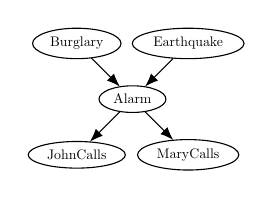
\begin{tikzpicture}[node distance=2cm,scale=0.5,every node/.style={scale=0.5}]
          \node[draw,ellipse] (alarm) {Alarm};
          \node[draw,ellipse,above left of=alarm] (burglary) {Burglary};
          \node[draw,ellipse,above right of=alarm] (earthquake) {Earthquake};
          \node[draw,ellipse,below left of=alarm] (johnCalls) {JohnCalls};
          \node[draw,ellipse,below right of=alarm] (maryCalls) {MaryCalls};
          \draw[-Latex] (burglary) -- (alarm);
          \draw[-Latex] (earthquake) -- (alarm);
          \draw[-Latex] (alarm) -- (johnCalls);
          \draw[-Latex] (alarm) -- (maryCalls);
        \end{tikzpicture}
      \end{block}
      \vspace{1cm}
      \begin{block}{Markov Random Field}
        \centering
        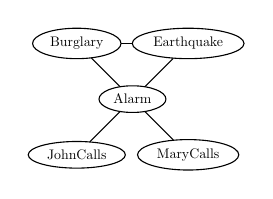
\begin{tikzpicture}[node distance=2cm,scale=0.5,every node/.style={scale=0.5}]
          \node[draw,ellipse] (alarm) {Alarm};
          \node[draw,ellipse,above left of=alarm] (burglary) {Burglary};
          \node[draw,ellipse,above right of=alarm] (earthquake) {Earthquake};
          \node[draw,ellipse,below left of=alarm] (johnCalls) {JohnCalls};
          \node[draw,ellipse,below right of=alarm] (maryCalls) {MaryCalls};
          \draw (burglary) -- (earthquake);
          \draw (burglary) -- (alarm);
          \draw (earthquake) -- (alarm);
          \draw (alarm) -- (johnCalls);
          \draw (alarm) -- (maryCalls);
        \end{tikzpicture}
      \end{block}
    \end{column}
  \end{columns}
  \onslide<2>{
    \begin{tikzpicture}[remember picture,overlay]
      \node[draw,star,fill=red!10] (wmc) at (current page.center) {WMC};
      \coordinate[xshift=-0.25\linewidth,yshift=-0.25\textheight] (p1) at (current page.center);
      \coordinate[xshift=0.25\linewidth,yshift=-0.25\textheight] (p2) at (current page.center);
      \coordinate[xshift=-0.25\linewidth,yshift=0.25\textheight] (p3) at (current page.center);
      \coordinate[xshift=0.25\linewidth,yshift=0.25\textheight] (p4) at (current page.center);
      \draw[-latex,line width=2pt,color=red!50] (p1) -- (wmc);
      \draw[-latex,line width=2pt,color=red!50] (p2) -- (wmc);
      \draw[-latex,line width=2pt,color=red!50] (p3) -- (wmc);
      \draw[-latex,line width=2pt,color=red!50] (p4) -- (wmc);
    \end{tikzpicture}
  }
\end{frame}

\begin{frame}[fragile]{Weighted Model Counting (WMC)}
  \begin{columns}
    \begin{column}{0.5\textwidth}
      \begin{itemize}
      \item Generalises propositional model counting ($\#\SAT{}$)
      \item Applications:
        \begin{itemize}
        \item graphical models
        \item probabilistic programming
        \item neural-symbolic artificial intelligence
        \end{itemize}
      \item Main types of algorithms:
        \begin{itemize}
        \item using knowledge compilation
        \item using a \SAT{} solver
        \item manipulating pseudo-Boolean functions
        \end{itemize}
      \end{itemize}
    \end{column}
    \begin{column}{0.5\textwidth}
      \begin{example}
      $w(x) = 0.3$, $w(\neg x) = 0.7$, $w(y) = 0.2$, $w(\neg y) = 0.8$
      \vspace{1cm}

      $\mathsf{WMC}(\alert{x \lor y}) = w(x)w(y) + w(x)w(\neg y) + w(\neg x)w(y)
      = 0.44$
      \end{example}
    \end{column}
  \end{columns}
\end{frame}

\begin{frame}[fragile]{The Problem with Assigning Weights to Literals}
  \begin{columns}[t]
    \begin{column}{0.5\textwidth}
      \begin{block}{A Simple Bayesian Network}
        \centering
        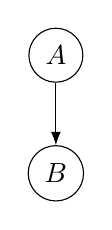
\begin{tikzpicture}[edge from parent/.style={draw,-{Latex}}]
          \node[draw,circle] at (0, 0) (a) {$A$}
          child {node[draw,circle] (b) {$B$}};
        \end{tikzpicture}
      \end{block}
      \begin{itemize}
      \item from \structure{2 binary} variables
      \item to \structure{8} variables and \structure{17} clauses
      \item with lots of redundancy
      \end{itemize}
    \end{column}
    \begin{column}{0.5\textwidth}
      \begin{block}{Its WMC Encoding}
        \vspace{-0.2cm}
\begin{lstlisting}[basicstyle=\scriptsize,escapeinside={(*}{*)},name=codeL]
p cnf 8 17
(*\only<2->{\aftergroup\speciallstcolor}*)-2 -1 0(*\only<2->{\aftergroup\endspeciallstcolor}*)
(*\only<2->{\aftergroup\speciallstcolor}*)1 2 0(*\only<2->{\aftergroup\endspeciallstcolor}*)
(*\only<2->{\aftergroup\speciallstcolortwo}*)-3 1 0(*\only<2->{\aftergroup\endspeciallstcolortwo}*)
(*\only<2->{\aftergroup\speciallstcolortwo}*)-1 3 0(*\only<2->{\aftergroup\endspeciallstcolortwo}*)
(*\only<2->{\aftergroup\speciallstcolorthree}*)-5 -1 0(*\only<2->{\aftergroup\endspeciallstcolorthree}*)
(*\only<2->{\aftergroup\speciallstcolorthree}*)-5 -4 0(*\only<2->{\aftergroup\endspeciallstcolorthree}*)
(*\only<2->{\aftergroup\speciallstcolorthree}*)1 4 5 0(*\only<2->{\aftergroup\endspeciallstcolorthree}*)
(*\only<2->{\aftergroup\speciallstcolorfour}*)-6 -1 0(*\only<2->{\aftergroup\endspeciallstcolorfour}*)
(*\only<2->{\aftergroup\speciallstcolorfour}*)-6 4 0(*\only<2->{\aftergroup\endspeciallstcolorfour}*)
(*\only<2->{\aftergroup\speciallstcolorfour}*)-4 1 6 0(*\only<2->{\aftergroup\endspeciallstcolorfour}*)
(*\only<2->{\aftergroup\speciallstcolorfive}*)-7 1 0(*\only<2->{\aftergroup\endspeciallstcolorfive}*)
(*\only<2->{\aftergroup\speciallstcolorfive}*)-7 -4 0(*\only<2->{\aftergroup\endspeciallstcolorfive}*)
(*\only<2->{\aftergroup\speciallstcolorfive}*)-1 4 7 0(*\only<2->{\aftergroup\endspeciallstcolorfive}*)
(*\only<2->{\aftergroup\speciallstcolorsix}*)-8 1 0(*\only<2->{\aftergroup\endspeciallstcolorsix}*)
(*\only<2->{\aftergroup\speciallstcolorsix}*)-8 4 0(*\only<2->{\aftergroup\endspeciallstcolorsix}*)
(*\only<2->{\aftergroup\speciallstcolorsix}*)-4 -1 8 0(*\only<2->{\aftergroup\endspeciallstcolorsix}*)
(*\only<2->{\aftergroup\speciallstcolorseven}*)-4 0(*\only<2->{\aftergroup\endspeciallstcolorseven}*)
c weights 1.0 1.0 0.5 1.0 \
0.5 1.0 1.0 1.0 0.6 1.0 \
0.4 1.0 0.1 1.0 0.9 1.0
\end{lstlisting}
        \vspace{-0.2cm}
      \end{block}
    \end{column}
  \end{columns}
  \only<2->{
    \begin{tikzpicture}[overlay,use tikzmark]
      \node[above right = 0 and 15 mm of pic cs:line-codeL-3-end] {\color{color1}{$\neg x_1 \Leftrightarrow x_2$}};
      \node[above right = 0 and 15 mm of pic cs:line-codeL-5-end] {\color{color2}{$x_1 \Leftrightarrow x_3$}};
      \node[above right = 0.5 ex and 10 mm of pic cs:line-codeL-8-end] {\color{color3}{$\neg x_1 \land \neg x_4 \Leftrightarrow x_5$}};
      \node[above right = 0.5 ex and 10 mm of pic cs:line-codeL-11-end] {\color{color4}{$\neg x_1 \land x_4 \Leftrightarrow x_6$}};
      \node[above right = 0.5 ex and 10 mm of pic cs:line-codeL-14-end] {\color{color5}{$x_1 \land \neg x_4 \Leftrightarrow x_7$}};
      \node[above right = 0.5 ex and 10 mm of pic cs:line-codeL-17-end] {\color{color6}{$x_1 \land x_4 \Leftrightarrow x_8$}};
      \node[above right = -0.5 ex and 20 mm of pic cs:line-codeL-18-end] {\color{color7}{$\neg x_4$}};
    \end{tikzpicture}
  }
\end{frame}

\begin{frame}
  \frametitle{Outline}
  \tableofcontents
\end{frame}

\section{An Alternative Formulation}
% TODO: Definition of WMC and MC-WMC

\begin{frame}{Formalising the Intuition from Before}
  For any propositional formula \structure{$\phi$} over a set of variables
  \structure{$X$} and \structure{$p, q \in \mathbb{R}$}, let
  \structure{$[\phi]^p_q\colon 2^X \to \mathbb{R}$} be the pseudo-Boolean
  function defined as
  \[
    [\phi]^p_q(Y) \coloneqq
    \begin{cases}
      p & \text{if } Y \models \phi \\
      q & \text{otherwise}
    \end{cases}
  \]
  for any \structure{$Y \subseteq X$}.

  \begin{definition}[Pseudo-Boolean Projection (PBP)]
    A \alert{PBP instance} is a tuple \structure{$(F, X, \omega)$}, where
    \structure{$X$} is the set of variables, \structure{$F$} is a set of
    two-valued pseudo-Boolean functions \structure{$2^X \to \mathbb{R}$}, and
    \structure{$\omega \in \mathbb{R}$} is the scaling factor.
  \end{definition}
\end{frame}

\begin{frame}{From WMC to PBP}
  \begin{example}
    \begin{itemize}
    \item Indicator variable: \structure{$x$}
    \item Parameter variables: \structure{$p$}, \structure{$q$}
    \item Weights: \structure{$w(p) = 0.2$}, \structure{$w(q) = 0.8$}, and \structure{$w(\neg p) = w(\neg q) = 1$}
    \end{itemize}
    \begin{center}
      \begin{tabular}{llll}
        \toprule
        WMC Clause & \onslide<2->{In CNF} & \onslide<3->{Pseudo-Boolean Function} & \\
        \midrule
        $\neg x \Rightarrow p$ & \onslide<2->{$x \lor p$} & \onslide<3->{$[\neg x]_1^{0.2}$} & \\
        $p \Rightarrow \neg x$ & \onslide<2->{$\neg x \lor \neg p$} & & \onslide<4->{$[x]^{0.8}_{0.2}$} \\
        $x \Rightarrow q$ & \onslide<2->{$\neg x \lor q$} & \onslide<3->{$[x]_1^{0.8}$} & \\
        $q \Rightarrow x$ & \onslide<2->{$x \lor \neg q$} & & \\
        $\neg x$ & \onslide<2->{$\neg x$} & \onslide<3->{$[\neg x]_0^1$} & \onslide<4->{$[\neg x]_0^1$} \\
        \bottomrule
      \end{tabular}
    \end{center}
  \end{example}
\end{frame}

\section{Correctness}

\section{Experimental Results}

\begin{frame}{Experimental Results}
  \centering
  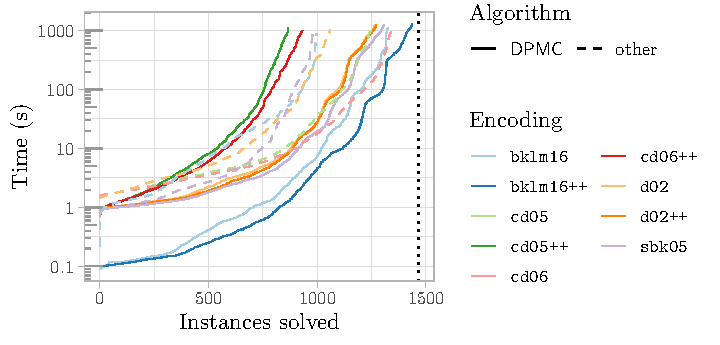
\includegraphics[width=\textwidth]{cumulative}
\end{frame}

\begin{frame}{Experimental Results}
  \centering
  \includegraphics[width=\textwidth]{scatter1}
\end{frame}

\begin{frame}{Experimental Results}
  \centering
  \includegraphics[width=\textwidth]{scatter2}
\end{frame}

\begin{frame}{Experimental Results}
  \centering
  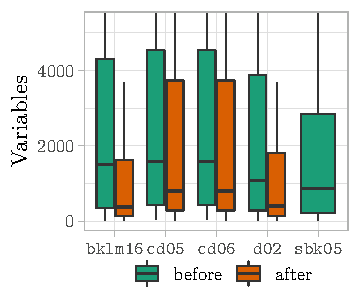
\includegraphics[width=\textwidth]{box}
\end{frame}
% TODO: fit the plot to the left half of the slide, add observations on the
% right

\section{Summary}

\begin{frame}{Summary}
\end{frame}

\end{document}